% Figure from MATH 591 notes, section 67. Added, not from lecture (Lecture 24): the half-line example.
\begin{tikzpicture}[scale=0.95]
\draw[thick, ->] (-5,0) -- (0,0);
\draw[thick, fill=white] (0,0) circle (2pt) node[below=2pt, font=\scriptsize] {$0$};
\node[font=\scriptsize, anchor=east] at (-5.05,0) {$M = (-\infty, 0)$};
\fill (-2.6,0) circle (1.5pt) node[below=2pt, font=\scriptsize] {$x_0$};
\foreach \x in {-4.4,-3.4,-1.6,-0.8} { \draw[->, blue!70!black, thick] (\x,0.25) -- (\x+0.45,0.25); }
\draw[blue!70!black, |-, thick] (-2.6,-0.55) -- (-0.03,-0.55);
\node[blue!70!black, font=\scriptsize, below] at (-1.3,-0.6) {$\varphi_t(x_0) = x_0 + t$ reaches $0$ at $t = -x_0$};
\node[font=\scriptsize, above] at (-2.6,0.45) {$\mathbf{X} = \dfrac{d}{dx}$};
\end{tikzpicture}
